%File: formatting-instruction.tex
\documentclass[letterpaper]{article}
% AAAI format packages
\usepackage{aaai}
\usepackage{times}
\usepackage{helvet}
\usepackage{courier}
% Additional packages
\usepackage{amsmath}
\usepackage{amssymb}
\usepackage{amsthm}
\usepackage{algorithm}
\usepackage{algorithmic}
\usepackage{graphicx}
\newtheorem{thm}{Theorem}
\newtheorem{defn}{Definition}
% END Additional packages
\frenchspacing
\setlength{\pdfpagewidth}{8.5in}
\setlength{\pdfpageheight}{11in}
\pdfinfo{
/Title (Experience-Biased Symbolic Planning)
/Author (Aram Ebtekar, Mike Phillips, Sven Koenig, Maxim Likhachev)
/Keywords (symbolic planning, E-graph, experience-biasedh, A* search, STRIPS, HSP)
}
\setcounter{secnumdepth}{0}  
 \begin{document}
% The file aaai.sty is the style file for AAAI Press 
% proceedings, working notes, and technical reports.
%
\title{Experience-Biased Symbolic Planning}
\author{Aram Ebtekar$^\dagger$ \and Mike Phillips$^\dagger$ \and Sven Koenig\thanks{University of Southern California, Los Angeles, CA 90089} \and Maxim Likhachev% <-this % stops a space
\thanks{Carnegie Mellon University, Pittsburgh, PA 15217}% <-this % stops a space
%
}
\maketitle
\begin{abstract}
\begin{quote}
Weighted A* search is the foundation for state-of-the-art domain-independent symbolic planners.
An important open challenge for these planners is to utilize experience with similar planning problems to speed up subsequent planning episodes.
Experience graphs have recently shown promise as a technique for plan reuse in the context of weighted A* searches in robotics, by biasing them towards a subgraph of the search space, typically chosen to consist of the edges used in previous plans.
In this paper, we demonstrate how to augment symbolic planners with
experience graphs, using the HSP2 planner as a representative
example.
The resulting planners are able to trade off seamlessly
between plan quality and runtime and thus have advantages over past
plan-reuse techniques, such as planning by analogy.
We demonstrate
experimentally that our planner speeds up HSP2 by a factor of 2 or more on
many domains while achieving about the same plan quality.
\end{quote}
\end{abstract}

\section{Introduction}
Planning entails finding action sequences that achieve a goal state.
In order to apply the language of graph theory, states are often thought of as nodes connected by action transitions.
A \textbf{plan} is a path from the start state to one of many goal states.
Despite the existence of classic polynomial-time search techniques, such as Dijkstra's algorithm, planning remains the crux of many difficult problems in AI.

The reason usually is that the graphs involved are very large; indeed, too large for explicit storage.
In motion planning, the state space may be a continuous geometric set whose desired discretization is very fine.
In symbolic planning, a planning language such as STRIPS, SAS+, ADL or PDDL [CITE] is chosen to give a compressed symbolic representation.

The graph is exponentially larger than its encoding so, in both cases, states are generated only as needed.
The symbolic representation sometimes encodes exploitable structure.
In order to create a domain-independent solver for a language such as STRIPS, we need to automatically extract and interpret structural information about the problem. 

In forward weighted A* search, a frontier of nodes expands from the start until it hits a goal, at which point a solution is found.
Rather than blindly searching the entire exponential-sized space, A* tries to focus toward the goal by expanding nodes which seem likely to lie on a short solution path.
The minimum length of a solution passing through a given frontier node is the sum of distances from the start to this node, and from this node to a goal.
The better we estimate these, the sooner we'll reach a solution.

Since A* expands in a fairly conservative fashion from the start state onward, the start-to-frontier estimates are very well-approximated by construction of a valid path.
Thus, the principal issue is the derivation of frontier-to-goal estimates.
Given exact distances, it would be a simple matter to trace a valid path from the start, taking optimal successors at each step, until a goal is reached.
In practice, we are forced to use estimates, which sometimes mislead us into local optima, wasting time on dead-end nodes.

These distance approximations are called \textbf{heuristics}, and we use them in hopes of finding good plans more efficiently.
Algorithms such as A* are designed to find solutions quickly whenever the heuristic is of reasonable quality.
If we hope to take subexponential time, we can only afford to examine a vanishing fraction of the states, and it is only for these that we compute the heuristic.
If the heuristic is good, we hope not to have to visit (i.e. generate) too many states.
Hence, there is a tradeoff between spending more time to compute a more accurate heuristic, vs evaluating a weaker heuristic quickly but at many more states.

In practice, even using state-of-the-art methods to generate heuristics on isolated planning instances, STRIPS problems can be very difficult to solve without expert domain knowledge.
Even humans have difficulty when faced with an unfamiliar kind of puzzle, though we get better with experience.
Thus, one might hope that a planning agent would similarly learn to generalize solutions from past planning experiences to related new instances.

A recent approach builds \textbf{experience graphs} to estimate the high-level connectivity of the free space in motion planning tasks \cite{phillips2012graphs}.
The intuition is to remember previously generated paths so that, when a new start and goals are queried, a new path can be quickly generated by reusing subpaths from the E-graph.
A variant of weighted A* is employed which biases its focus toward the E-graph.
While this work demonstrates promising results in robot motion planning, E-graphs have never before been applied to symbolic domain representations such as the STRIPS language.

Our present contribution is to investigate the use of E-graphs in STRIPS domains. In particular, we take the HSP2 planner \cite{bonet2001planning} as a representative of the class of modern weighted A* based symbolic planners, and augment its heuristic with a bias toward its E-graph. After presenting the related works, we begin by describing the STRIPS language and the original HSP heuristic. In the following section, we formally introduce E-graphs in technical detail. Then we combine the two approaches, resulting in the new Experience-Biased HSP planner. We present the algorithm and discuss its theoretical properties. This is followed by experiments showing promise for the application of E-graphs to symbolic problem solving. Finally, we conclude with some thoughts on extensions worth investigating.

\section{Related Work}

Classically, case-based reasoning methods 
such as PRIAR~\cite{Kamb:92}, SPA~\cite{Hank:95}, MRL~\cite{Koeh:94}, and NoLimit~\cite{mljournal}
have been used recall 
previous plans that appear similar to the current problem and 
then adapt them to meet the new specifications.
Compared to these methods, our work reuses prior experience in
the context of modern weighted A* methods. We also provide
a bound on the suboptimality of the solution. 

Recently there has been work on incorporating prior knowledge 
into modern planners (based on weighted A* and powerful heuristics).
For instance, GPG~\cite{Gere:00} uses planning graphs to adapt a prior path to the 
new scenario by searching locally within windows around plan 
inconsistencies. To guarantee completeness, the windows can grow 
if solutions are not found until they contrain the whole plan.
In this work~\cite{DBLP:conf/iccbr/RosaOB07} case-based reasoning is used to choose the 
order of state evaluations of EHC (enforced hill-climbing) which 
is a component in modern planners such as FF. 

OAKplan~\cite{Serina:2010:KFC:1860143.1860472} is a recent 
case-based reasoning method which converts 
planning instances to into a compact graph representation and 
then uses recent kernel methods for matching labeled graphs to select
a similar case to the problem at hand. The selected case is then 
adapted using LPG-ADAPT~\cite{Fox06planstability} LPG-ADAPT is a replanning method 
encourages \textit{plan stability}, which tries to make 
sure that the new plan is as similar to the previous plan as possible. 
The method also uses a modern heuristic search approach.

ERRT-PLAN~\cite{workshop-icaps12-errtplan} presents a very different 
approach to reuse in planning. 
Similar to E-Graphs, ERRT has its roots in motion planning~\cite{Bruce:2002}.
ERRT-PLAN applies this sampling-based motion planner that leverages 
reuse to symbolic planning. The planner randomly chooses to extend 
the search tree toward the goal, toward goals from previous 
plans, or to reuse an action from a previous plan. 
The extension operations are based on modern heuristic search
planners.
The stochastic nature of the direction the search progresses toward
allows it to overcome local minima caused by misleading heuristics.

The primary difference between our approach and previous ones 
is that we plan with prior experience in a way that have provable
bounds on suboptimality of the solution. The use of E-Graphs also
allows us to formulate this in a way that the user has control over
this suboptimality bound with an intuitive parameter that trades
reuse (speed) for solution quality.

\section{Old version of related works (to delete)}

A lot of symbolic planners that have emerged in recent years are based on forward weighted A* search. This paper focuses on HSP2 as a representative example, because it is fairly simple and embodies the core ideas common to many state-of-the-art planners. The use of E-graphs is orthogonal to many of the latest improvements, so our methods can in principle be adapted to any A* planner.

HSP2 is based on the HSP planner [CITE] which performed well in the AIPS-98 planning competition. HSP combined a novel heuristic with a hill-climbing algorithm. HSP2 used the same heuristic, but with a weighted A* search, and produced even better results. FF and GRT develop these heuristics further.

Fast Downward \cite{helmert2006fast} is a planner that decomposes planning tasks using a contruct called the causal graph heuristic. The LAMA planner \cite{richter2010lama}, which won the International Planning Competition 2008, replaces the causal graph with landmark heuristics.

While many of these planners perform preprocessing in an attempt to automatically extract knowledge about the domain, none are capable of using their own fully generated plans to inform later searches. A few works were made in similar directions, for example \cite{fikes1972learning} are able to generalize their plans, \cite{veloso1992learning} is able to relate by analogy to known solutions, and \cite{borrajo2012probabilistically} probabilistically chooses whether to step along past plans or explore new paths.

\section{STRIPS Language}

A STRIPS problem is a tuple $P = \langle A,O,I,G\rangle$ consisting of an atom set $A$, operator set $O$, initial state $I \subseteq A$ and goal condition $G \subseteq A$.
Each operator $op\in O$ is defined by its cost, preconditions, add effects and delete effects: $Cost(op) \in \mathbb{R}^+$ and $Prec(op),Add(op),Del(op) \subseteq A$.

The problem $P$ defines a directed state graph $(V,c)$ where $V$ is the power set of $A$ (i.e. states $S\in V$ correspond to collections of atoms), and the edge costs are
\begin{eqnarray*} c(S,S') = \min\{Cost(op) \mid S\supseteq Prec(op)\text{ and}
\\S' = \left(S \setminus Del(op)\right) \cup Add(op)\} \end{eqnarray*}
%consists of states transitions $(u,v)$ for which there exists an operator $op\in O$ with $u\in Prec(op)$ and $v = u - Del(op) \cup Add(op)$; the weight of this edge is the minimum cost of such an $op$.
By default, $c(S,S') = \infty$ when there is no operator directly transitioning from $S$ to $S'$.
Given a STRIPS problem $P$, we seek a low-cost path from the initial state $I\in V$ to any of the goal states $S\in V$ such that $S \supseteq G$. In this paper, we are particularly concerned with sequences of problems in which $A$ and $O$ are fixed, but various pairs $\langle I,G\rangle$ are queried.

\section{HSP Heuristic}

Many of today's state-of-the-art domain-independent STRIPS planners are based on the HSP2 planner \cite{bonet2001planning}, which we now describe.
It's common to compute heuristics by solving an easier, relaxed version of the original problem. In STRIPS, one might ignore the delete lists of operations.
Since having more atoms makes preconditions and the goal condition more likely to hold, this can only make the problem easier, so the resulting heuristic never overestimates the true cost.

However, even the relaxed STRIPS planning problem includes set-cover as a special case, making it NP-hard.
Intuitively, we see that the relaxed search space remains exponential.
To reduce it, HSP2 decouples the atoms, instead estimating the cost of achieving each individual atom.

Let's say we want a heuristic estimate of the distance from $S$ to a goal that contains $G$. HSP2 estimates the cost to achieve an atom $a\in A$ from $S$ by $g_S(a) = $
\[\begin{cases} 0  &\mbox{if } a \in S
\\ \min_{op\mid a\in Add(op)} \left(g_S(Prec(op)) + Cost(op)\right)  &\mbox{if } a \notin S \end{cases}\]

The HSP heuristic (also used in HSP2) is then defined by
\[h^{HSP}(S) = g_S(G),\]
the estimated cost of achieving all atoms in $G$. Note that $g_S(\cdot)$ is evaluated on certain atom sets, namely $Prec(op)$ and $G$.
To keep the computations feasible, define $g_S(P) = \max_{p\in P} g_S(p)$ for atom sets $P$.
The resulting HSP-max heuristic is an underestimate; indeed, it satisfies a stronger property called \textbf{consistency}.

\begin{defn} For $\epsilon\ge 1$, a heuristic $h$ is called \textbf{$\epsilon$-consistent} if $h(S) = 0$ when $S$ is a goal and $h(S) \le \epsilon c(S,S') + h(S')$ for all $S,S'\in V$. $h$ is \textbf{consistent} if it is $1$-consistent. \end{defn}
\begin{thm} Given an $\epsilon$-consistent heuristic and expanding no node more than once, A* is guaranteed to find a path costing no more than $\epsilon$ times the optimal path cost \cite{LikGorThr-ara}. \end{thm}

If the atoms were truly independent, a more accurate estimate would be $g_S(P) = \sum_{p\in P} g_S(p)$.
Despite its inconsistency in general, the latter HSP-plus heuristic is often useful in practice, as it uses more information and biases more greedily toward the goal.

From a computational perspective, the HSP heuristic must compute $g_S(a)$ for all $a\in A$ whenever a new state $S$ is generated.
This can be done by dynamic programming, iterating the recursive formula to a fixpoint in Bellman-Ford-like fashion.
Pseudocode is listed in Algorithm \ref{alg:ComputeG}.

\begin{algorithm}
\caption{ComputeG($S$)}
\label{alg:ComputeG}
\begin{algorithmic}
\FORALL{$a \in A$}
\IF{$a \in S$}
\STATE $g_S(a) \leftarrow 0$
\ELSE
\STATE $g_S(a) \leftarrow \infty$
\ENDIF
\ENDFOR
\REPEAT
\FORALL{$op \in O$}
\STATE $cost\_estimate \leftarrow g_S(Prec(op)) + Cost(op)$
\FORALL{$a \in Add(op)$}
\STATE $g_S(a) \leftarrow \min \left(g_S(a),~cost\_estimate\right)$
\ENDFOR
\ENDFOR
\UNTIL{no further change in $g_S$-values}
\end{algorithmic}
\end{algorithm}

In a sense, a lot of work is wasted by estimating the cost to reach every atom, when we only require $g_S(G)$.
Later, we'll see how to make better use of this computation.

\section{Experience Graphs}

E-graphs can improve total search time over a series of related queries on the same graph.
Formally, an E-graph is a subgraph of the state space.
We update it between queries, typically by adding the solution path from the previous search query.

Suppose we have a consistent heuristic $h(S,S')$ for the distance between arbitrary pairs of states.
That is, $h$ obeys the triangle inequality, is never dominated by an edge cost, and $h(S,S) = 0$ for all $S\in V$.
The E-graph heuristic $h^E$ biases the search to follow E-Graph edges instead of $h$ by penalizing the latter by an inflation factor $\epsilon^E > 1$.
To be precise, define

\[h^E(S_0) = \min_{N,S_N,\pi} \sum_{i=1}^N \min \{\epsilon^E h(S_{i-1},S_i),c^E(S_{i-1},S_i)\}\]
with the minimization taking place over all goal states $S_N$ and paths $\pi = \langle S_0,S_1,...,S_N \rangle$. $c^E$ are E-graph edge costs, or $\infty$ if the E-graph edge does not exist.

In the limit as $\epsilon^E \rightarrow 1$, E-graph edges offer no advantage as $h(S_{i-1},S_i) \le c^E(S_{i-1},S_i)$. Hence, using the triangle inequality to coalesce the sum,
\[h^E(S_0) = \min_{N,S_N,\pi} \sum_{i=1}^N h(S_{i-1},S_i) = \min_{S_N} h(S_0,S_N)\]

Conversely, as $\epsilon^E \rightarrow\infty$, the inflated terms dominate. Hence, the minimizing path becomes the one which incurs the least estimated cost outside the E-graph. In particular, $h^E$ has the following property:

\textit{For sufficiently large $\epsilon^E$, once the A* frontier touches an E-graph component which includes a goal state, no node outside the E-graph will ever again need to be expanded.}

This means, for instance, that if the E-graph already contains a path from the start to a goal, then A*, guided by $h^E$ with large bias parameter $\epsilon^E$, will never leave the E-graph.
If the E-graph is small, a solution would promptly be discovered.
In this manner, little work is needed to solve previously encountered subproblems.

We cannot afford to compute $h^E$ according to its literal definition, as there are far too many paths to consider.
Fortunately, there exists a practical means of computing it. By the triangle inequality, any consecutive pair of $h(S_{i-1},S_i)$ terms can be merged into one.
Thus, we lose no generality in restricting $S_i$ to lie on the E-graph for $0 < i < N$.
The heuristic computation can focus on the E-graph, using $h(S_{i-1},S_i)$ to estimate the cost of leaving the E-graph at $S_{i-1}$ before re-entering it at $S_i$.

Let $V^E$ be the union of the goal states and the E-graph's vertices.
In addition to following E-graph edges, we imagine it's possible to ``jump" from $S$ to $S'$ at cost $\epsilon^E h(S,S')$.
That is, let $c'(S,S') = \min\left(c^E(S,S'),~\epsilon^E h(S,S')\right)$


In a preprocessing stage before the main search, we apply Dijkstra's algorithm once in reverse with the costs $c'$ to compute the estimated distance-to-goal $h^E(S)$ from every $S\in V^E$. Ignoring the computation of $h$ (presently considered as a blackbox), this preprocessing takes $O(|V^E|^2)$ time, which is insignificant for small E-graphs and goal sets.

Later, when generating $S \notin V^E$, we see that we have already precomputed costs of paths consisting of all but the first edge of $\pi$ according to the definition of $h^E(S)$. Thus, we derive the mathematically equivalent but much cheaper computation
\[h^E(S) = \min_{S'\in V^E} \left(\epsilon^E h(S,S') + h^E(S')\right)\]

\begin{thm}$h^E$ is $\epsilon^E$-consistent. \cite{phillips2012graphs}\end{thm}

\begin{figure}
	\begin{center}
	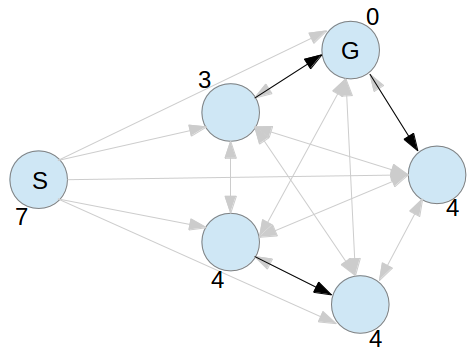
\includegraphics[scale=0.5]{Pentagon.png}
	\end{center}
	\caption{An example E-graph and corresponding heuristic computations.}
	\label{fig:example}
\end{figure}

Figure \ref{fig:example} illustrates the idea. Suppose the dark edges have cost 3 and make up the E-graph. Off-E-graph edges are not shown, as they are only accessed indirectly via $h$; instead, light edges represent the jump estimates $h(S_i,S_j) = 2$ (with one exception: $h(S,G) = 5$), which we inflate by a factor $\epsilon^E=2$ to make 4 (or 10, respectively). Dijkstra's algorithm follows dark and light edges backward to compute the $h^E$ values shown alongside each node.

$G$ is on the E-graph, though this need not be the case in general. $V^E$ is the pentagon on the right, and its $h^E$ values are precomputed before the search. For $S\notin V^E$, $h^E(S)$ is computed only when A* generates $S$.

\section{Experience-Biased HSP}

Now we combine the ideas from HSP2 and E-graphs to construct a domain-independent STRIPS planner which learns from experience. In STRIPS, a consistent heuristic $h(S,S')$ is given by the HSP-max estimate $g_S(S')$. We can compute $g_S(S')$ for all $S,S'\in V^E$ in precisely $|V^E|$ runs of Algorithm \ref{alg:ComputeG}: each run provides us with $|V^E|$ of these results, yielding $(|V^E|)^2$ values in total.

As before, Dijkstra's algorithm combines an inflation of these estimates with the E-graph edges to derive $h^E(S)$ for all $S\in V^E$. Note that in STRIPS, $V^E$ need not include every goal state: the minimal goal $G$ suffices as it's always the easiest to reach in the heuristic relaxation.

Upon encountering a new state $S\notin V^E$, we run Algorithm \ref{alg:ComputeG} again to compute $g_S(a)$ for all atoms $a\in A$. Then it's a simple matter to compute the E-graph heuristic by

\[h^E(S) = \min_{S'\in V^E} \left( \epsilon^E g_S(S') + h^E(S') \right)\]

We remark that, when E-graphs are involved, the values $g_S(S')$ on the right-hand side range over a variety of different states $S'$. Compare this to the formula for $h^{HSP}$, which uses only $g_S(G)$. HSP2 would still compute all the $g_S$-values despite using them only once, so here we get to consult the E-graph essentially for free. The only additional work is the minimization over $S'\in V^E$, which takes O($|V^E||A|$) time. A pseudocode implementation is listed in Algorithm \ref{alg:Search}. The parameter $\epsilon^E$ controls bias toward the E-graph, while the weight $\epsilon$ provides a uniform goal-directed bias.

\begin{algorithm}
\caption{Search()}
\label{alg:Search}
\begin{algorithmic}
\FORALL{$S \in V^E$}
\STATE ComputeG($S$)
\FORALL{$S' \in V^E$}
\STATE $c'(S,S') \leftarrow \min\left(c^E(S,S'),~\epsilon^E g_S(S')\right)$
\ENDFOR
\ENDFOR
\STATE Compute $h^E$ on $V^E$ by reverse Dijkstra from $G$ with $c'$.
\STATE Run A* on the full graph from $I$ with heuristic $\epsilon h^E$:
\FOR{$S \notin V^E$ when generated by A*}
\STATE ComputeG($S$)
\STATE $h^E(S) \leftarrow \min_{S'\in V^E} \left( \epsilon^E g_S(S') + h^E(S') \right)$
\ENDFOR
\IF{A* successfully found a path to some goal state $S \supseteq G$}
\STATE Add all edges of the solution path to the E-graph.
\RETURN solution path
\ELSE
\RETURN failure
\ENDIF
\end{algorithmic}
\end{algorithm}

ComputeG($S$) implements the dynamic programming computation of $g_S$-values.
Each iteration of the outermost loop permanently fixes at least one $g_S(a)$ value, so it does at most $|A|+1$ iterations.
Multiplying nested loop iterations together and dropping cardinality signs for brevity, a conservative runtime bound on Algorithm \ref{alg:ComputeG} is $O(\mathbf{A^2O})$.
Thus, each state generated costs $O(\mathbf{A^2O + V^EA})$ time.

The preprocessing cost is $O(\mathbf{V^EA^2O + (V^E)^2A})$, asymptotically equivalent to preemptively generating every state in $V^E$.
In fact, most of the preprocessing requires no knowledge of $G$, so it can be done in advance of the new planning query. Once the query $\langle I,G\rangle$ is given, the remaining work consists of completing the $c'(S,G)$ computations from $g_S(a),a\in G$, and then running Dijkstra's algorithm from $G$. This costs only $O(\mathbf{V^E(A + V^E)})$ time.

For comparison, standard HSP2 without E-graphs takes $O(\mathbf{A^2O})$ time (with essentially the same constant factors) to generate each state, and does not incur the cost of generating a state unless the A* frontier encounters it.
When HSP2 is augmented with small E-graphs, the same asymptotic bound continues to hold, provided that the number of E-graph vertices is limited to $O(\mathbf{AO})$. Furthermore, we retain completeness and the ability to configure suboptimality bounds by adjusting the bias parameters:

\begin{thm}
Provided there exists a path from initial state $I$ to a goal state $S\supseteq G$, the experience-biased HSP algorithm finds a path which is at most $\epsilon\epsilon^E$-suboptimal.
\end{thm}

This follows directly from Theorems 1 and 2, since the weighted heuristic $\epsilon h^E$ is $\epsilon \epsilon^E$-consistent.
However, E-graphs make no guarantee of improving the search time. Indeed, biasing toward bad regions could trap the planner inside large local optima.
Potential gains depend entirely on choosing a good small set of edges to form our E-graph.
In our experiments, we simply keep the previous solution path; different choices remain a topic for future investigations.

Finally, we remark that the Experience-Biased HSP algorithm is highly parallelizable, even if A* is retricted to expanding nodes sequentially. Recall that the sum, min and max functions are computable in logarithmic time using linearly many processors. Therefore, with minor adjustments, ComputeG($S$) has parallel depth $O(\mathbf{A\log A\log O})$. With $\mathbf{A\max(O,V^E)}$ processors, the total cost of generating a state is $O(\mathbf{(A\log O + \log V^E)\log A})$. Using even more processors, the cost of \textit{expanding} a state can be reduced to the same by generating its successors in parallel. If still more processors are available, some may dedicate to the task of preemptively computing $h^E$ for states that are likely to be generated in the future, e.g. near the A* frontier.

\section{Experiment 1}

We augmented the original HSP2 planner code \cite{bonet2001planning} with E-graphs.
Since HSP-plus performs better in practice than HSP-max, we take the former heuristic as our baseline.
Our aim is to observe the planning time speedup achieved by applying E-graphs on a variety of STRIPS domains.
To measure this, we prepared two sets of experiments, of which this section describes the first.

In this experiment set, we solve several hundred problem instances across 18 domains taken from the HSP2 test suite.
For each problem, we first plan without experiences, using the HSP-plus heuristic in an A* search with weight $\epsilon=5$.
This search acts as our scientific \textbf{control}.
If the control fails to find a solution within 5 seconds, we discard the problem instance as being too difficult.
Otherwise, we record the plan cost and the number of states that were generated during the search.
Thus, we end up considering 321 problem instances.

For each of these, we run 3 additional searches using E-graphs, setting $\epsilon^E=5$ but reducing $\epsilon$ to 1, thus maintaining the same theoretical suboptimality bound.
The E-graphs consist of 20\%, 50\% and 80\% of the edges from the control's solution path, respectively, selected at random. For each of these, we again record the solution cost and number of nodes generated, and compare these figures to the control.
Define \textbf{speedup} as the ratio of the number of nodes generated in the control to the number generated in the E-graph search.
Likewise, define the \textbf{cost improvement} as the ratio of solution cost in the control to cost in the E-graph search.
We use nodes generated instead of time to produce deterministic results which are independent of most engineering details.
The times taken generally seemed to follow similar trends; as suggested by the analysis, the time spent per node changes little when small E-graphs are used.

The results are summarized in Figure \ref{tab:percent}.
We see that while performance in virtually unaffected in some domains, it's never substantially worsened, and in certain domains the experience helps greatly.
For example, results are strongly positive in the Blocks World.
Furthermore, figures [CITE numbers] show that the solution quality remains competitive; indeed, we see that when E-graphs are employed, the path cost is slightly reduced on average.

Note that saving 100\% of the E-graph would seem to trivially grant us the solution, as we could simply follow the remembered path depth-first.
In practice, since we fixed the bias parameter $\epsilon^E$ to 5 rather than raising it to an extremely large value, the search expands a fair number of states even if we remember most or all of the path.
This is necessary to ensure the suboptimality bound, as the planner does not know whether the E-graph can be ``trusted" to yield an efficient path.

\begin{figure}
	\begin{center}
	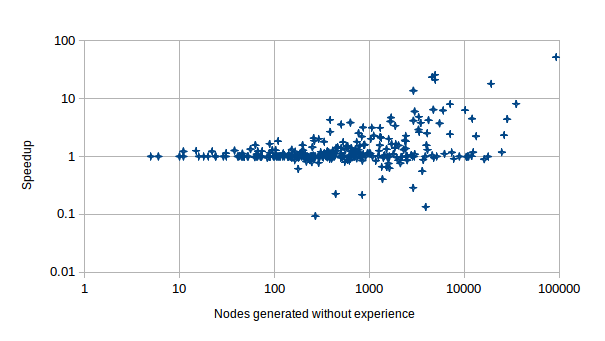
\includegraphics[scale=0.5]{Speedup_20_0.png}
	\end{center}
	\caption{20\% E-graph}
	 \label{fig:s_20_0}
\end{figure}

\begin{figure}
	\begin{center}
	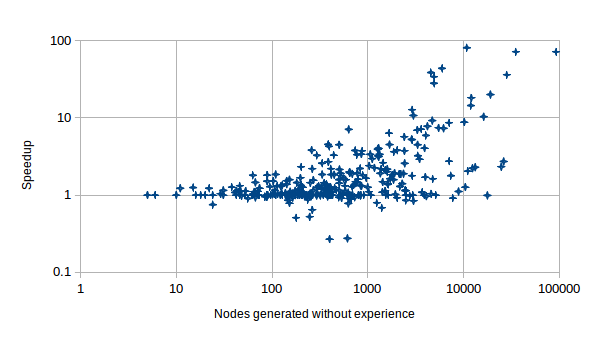
\includegraphics[scale=0.5]{Speedup_50_0.png}
	\end{center}
	\caption{50\% E-graph}
	 \label{fig:s_50_0}
\end{figure}

\begin{figure}
	\begin{center}
	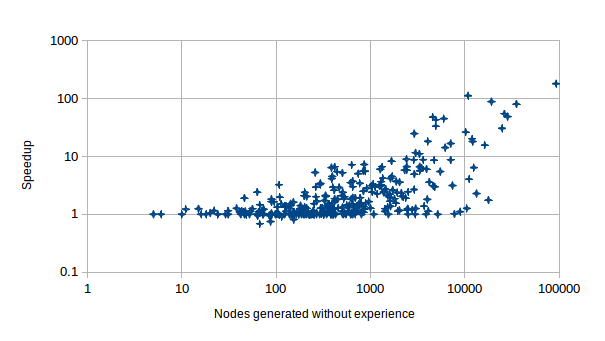
\includegraphics[scale=0.5]{Speedup_80_0.png}
	\end{center}
	\caption{80\% E-graph}
	 \label{fig:s_80_0}
\end{figure}

\begin{figure}
	\begin{center}
	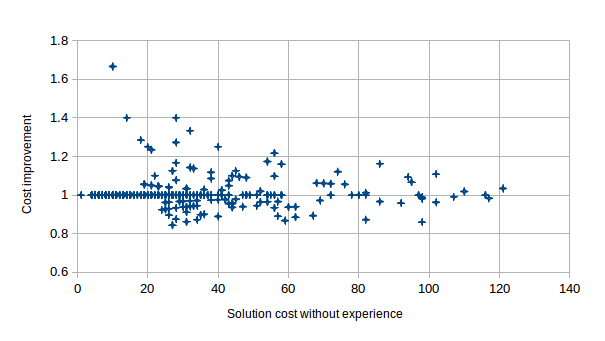
\includegraphics[scale=0.5]{Cost_20_0.png}
	\end{center}
	\caption{20\% E-graph}
	 \label{fig:c_20_0}
\end{figure}

\begin{figure}
	\begin{center}
	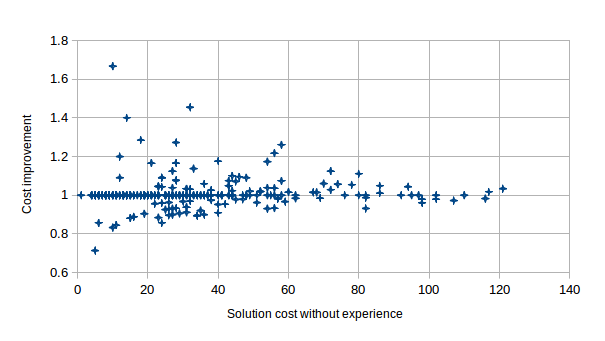
\includegraphics[scale=0.5]{Cost_50_0.png}
	\end{center}
	\caption{50\% E-graph}
	 \label{fig:c_50_0}
\end{figure}

\begin{figure}
	\begin{center}
	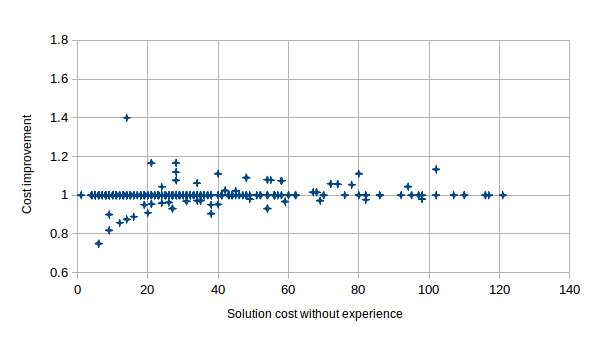
\includegraphics[scale=0.5]{Cost_80_0.png}
	\end{center}
	\caption{80\% E-graph}
	 \label{fig:c_80_0}
\end{figure}

\begin{table}
	\begin{center}
	    \begin{tabular}{| l | l | l | l | l |}
	    \hline
	    Domain & Inst & 20\% & 50\% & 80\%
	    \\ \hline
	    blocks & 35 & 1.08-1.82 & 1.37-3.73 & 1.90-5.84
	    \\ \hline
	    driverlog & 14 & 1.00-1.49 & 1.11-1.58 & 1.15-1.60
	    \\ \hline
	    elevators & 30 & 1.00-1.62 & 1.00-2.84 & 1.04-3.19
	    \\ \hline
	    freecell & 34 & 1.00-1.06 & 1.00-1.12 & 1.00-1.08
	    \\ \hline
	    grid & 2 & 1.07-1.18 & 2.16-3.57 & 2.22-3.75
	    \\ \hline
	    logistics00 & 28 & 0.91-1.04 & 0.98-1.13 & 1.03-1.19
	    \\ \hline
	    logistics98 & 5 & 0.95-1.01 & 1.09-1.62 & 1.24-3.00
	    \\ \hline
	    mprime & 19 & 1.00-1.00 & 1.00-1.07 & 1.00-2.46
	    \\ \hline
	    pegsolitaire & 29 & 1.00-3.57 & 1.13-4.49 & 1.68-6.63
	    \\ \hline
	    pipesworld-notankage & 15 & 1.00-3.27 & 1.00-7.07 & 1.00-9.95
	    \\ \hline
	    pipesworld-tankage & 8 & 1.00-1.00 & 1.00-1.02 & 1.00-1.45
	    \\ \hline
	    rovers & 13 & 0.97-1.23 & 1.23-7.09 & 1.23-7.17
	    \\ \hline
	    satellite & 16 & 0.99-1.00 & 1.00-1.26 & 1.00-1.26
	    \\ \hline
	    scananalyzer & 16 & 1.00-1.15 & 0.93-1.20 & 1.00-1.36
	    \\ \hline
	    sokoban & 11 & 1.12-2.10 & 1.32-3.02 & 1.56-7.80
	    \\ \hline
	    tpp & 10 & 1.00-1.00 & 1.00-1.23 & 1.00-2.31
	    \\ \hline
	    transport & 23 & 1.00-1.14 & 1.09-1.86 & 1.19-1.89
	    \\ \hline
	    zenotravel & 13 & 1.02-1.15 & 1.08-1.44 & 1.14-1.58
	    \\ \hline
	    TOTAL & 321 & 1.00-1.29 & 1.00-1.91 & 1.02-2.68
	    \\ \hline
	    \end{tabular}
	\end{center}
	\caption{Speedups for various E-graph \%s over various domains. Statistics are presented in the form (1st quartile)-(3rd quartile).}
	 \label{tab:percent}
\end{table}

\section{Experiment 2}

The previous experimental setup tested our ability to generalize from incomplete partial plans stored in memory; however, the new planning instances solved were identical to that used by the control to generate the E-graph.
Now, we try moving the start and goal nodes by having each of them take 5, 20 or 50 random walk steps in the state space. 
In this manner, we test how well E-graphs can generalize to nearby but non-identical queries.

We narrow our focus to 13 domains, and take from each of them the same set of instances as in the previous experiment, yielding 218 problem instances in all.
This time, we save 100\% of the solution path found by the control.
Then for each problem, we run 3 queries using this E-graph, moving each the start and goal by 5, 20 and 50 random steps, respectively.

Results are summarized in Figure \ref{fig:c_100_50}.
Again we observe encouraging speedups, though they decrease as we walk farther distances from the original query.

\begin{figure}
	\begin{center}
	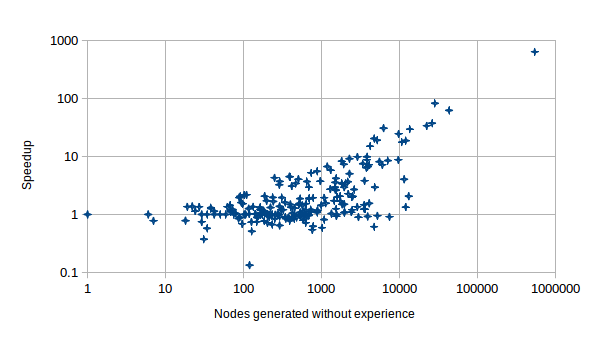
\includegraphics[scale=0.5]{Speedup_100_5.png}
	\end{center}
	\caption{5 random steps}
	 \label{fig:s_100_5}
\end{figure}

\begin{figure}
	\begin{center}
	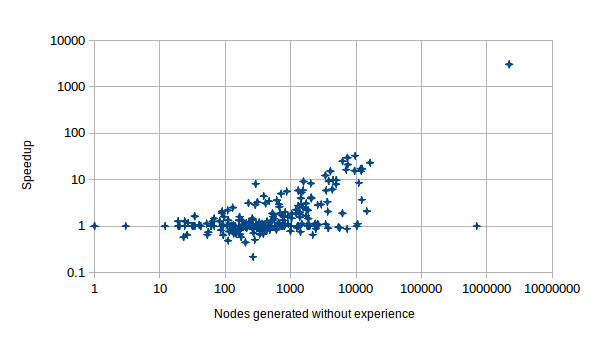
\includegraphics[scale=0.5]{Speedup_100_20.png}
	\end{center}
	\caption{20 random steps}
	 \label{fig:s_100_20}
\end{figure}

\begin{figure}
	\begin{center}
	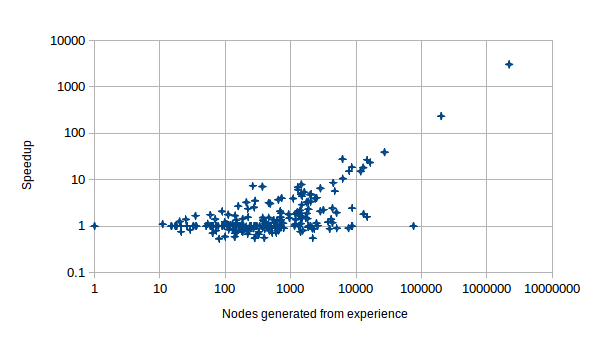
\includegraphics[scale=0.5]{Speedup_100_50.png}
	\end{center}
	\caption{50 random steps}
	 \label{fig:s_100_50}
\end{figure}

\begin{figure}
	\begin{center}
	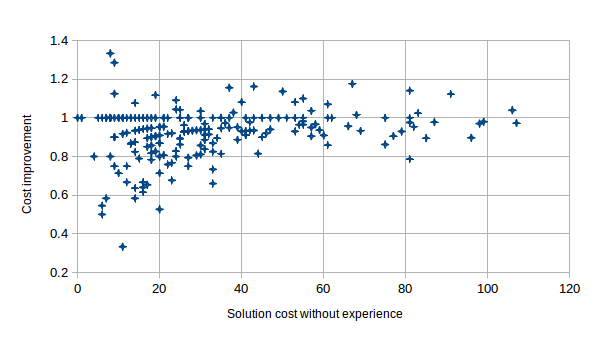
\includegraphics[scale=0.5]{Cost_100_5.png}
	\end{center}
	\caption{5 random steps}
	 \label{fig:c_100_5}
\end{figure}

\begin{figure}
	\begin{center}
	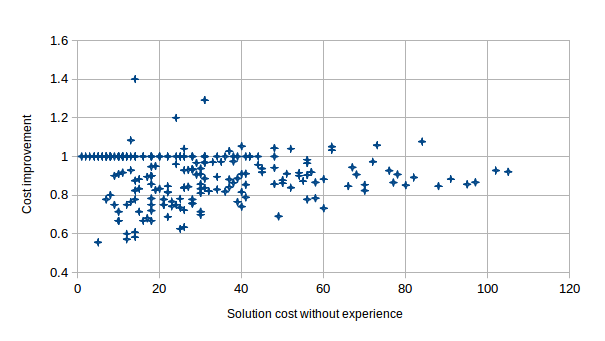
\includegraphics[scale=0.5]{Cost_100_20.png}
	\end{center}
	\caption{20 random steps}
	 \label{fig:c_100_20}
\end{figure}

\begin{figure}
	\begin{center}
	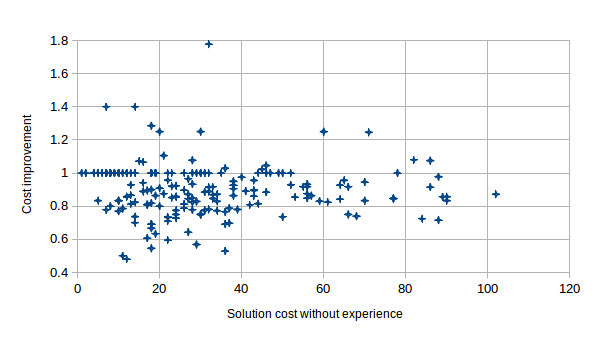
\includegraphics[scale=0.5]{Cost_100_50.png}
	\end{center}
	\caption{50 random steps}
	 \label{fig:c_100_50}
\end{figure}


\begin{table}
	\begin{center}
	    \begin{tabular}{| l | l | l | l | l |}
	    \hline
	    Domain & Inst & 5 steps & 20 steps & 50 steps
	    \\ \hline
	    blocks & 35 & 2.12-7.92 & 2.12-8.70 & 2.21-6.25
	    \\ \hline
	    driverlog & 14 & 0.86-2.42 & 0.85-1.30 & 0.82-1.20
	    \\ \hline
	    elevators & 30 & 1.09-4.04 & 0.99-2.76 & 0.90-2.06
	    \\ \hline
	    grid & 2 & 2.21-3.71 & 1.11-1.34 & 1.10-1.30
	    \\ \hline
	    logistics00 & 28 & 1.00-1.15 & 0.90-1.11 & 0.84-1.18
	    \\ \hline
	    logistics98 & 5 & 1.01-2.95 & 0.82-2.06 & 0.80-2.41
	    \\ \hline
	    pipesworld-notankage & 15 & 1.09-5.30 & 1.00-5.46 & 1.00-2.88
	    \\ \hline
	    pipesworld-tankage & 8 & 1.00-1.20 & 0.99-1.00 & 1.00-1.13
	    \\ \hline
	    rovers & 13 & 1.00-1.50 & 1.00-1.00 & 1.00-1.00
	    \\ \hline
	    satellite & 16 & 0.91-1.25 & 0.87-1.15 & 0.90-1.43
	    \\ \hline
	    scananalyzer & 16 & 0.74-1.52 & 1.00-1.00 & 1.00-1.00
	    \\ \hline
	    transport & 23 & 1.26-1.91 & 0.93-1.87 & 0.98-1.46
	    \\ \hline
	    zenotravel & 13 & 0.80-1.27 & 0.84-1.02 & 1.00-1.00
	    \\ \hline
	    TOTAL & 218 & 0.99-2.72 & 1.00-2.07 & 1.00-1.88
	    \\ \hline
	    \end{tabular}
	\end{center}
	\caption{Statistics are presented in the form (1st quartile)-(3rd quartile).}
	 \label{tab:walk}
\end{table}

\section{Analysis of HSPr (section to be deleted)}

Whether or not E-graphs are used, the call to ComputeG($S$) at each node generation is quite substantial. For this reason, a variant of HSP, called HSPr, searches the regression space of STRIPS, where each node represents a ``subgoal". The search proceeds backward from the goal. In this case, the heuristic must estimate the cost to achieve a given state $S$ (considered as a subgoal) from the initial state $I$. A single preprocessing call to ComputeG($I$) allows each $h^{HSPr}(S) = g_I(S)$ to be computed in $O(\mathbf{A})$ time.

With E-graphs, in backward as well as forward search, we call ComputeG($S$) for all $S\in V^E$; only now, $V^E$ includes $I$ instead of $G$. From $I$, a forward Dijkstra yields $h^E(S)$ for all $S\in V^E$. Then for $S\notin V^E$, the E-graph heuristic estimate of the cost from $I$ to $S$ is given by
\[h^E(S) = \min_{S'\in V^E}\left(h^E(S') + \epsilon^E g_{S'}(S) \right)\]

Since $g_{S'}$ was precomputed, the cost of generating a state is reduced to just $O(\mathbf{V^EA})$. Nonetheless, the overhead of using E-graphs is much more substantial in backward than in forward search, contributing a $|V^E|$ factor on the state generation cost.

Since a major benefit of backward HSP is being able to generate states in $O(\mathbf{A})$ time, it appears E-graphs in their present form are less likely to be of much help. However, in domains where forward search is more practical, we saw that E-graphs can effectively provide free hints.

\section{Conclusions (needs citations)}

We saw that by reusing pieces from past plans, E-graph-based planners can find solutions more quickly as they learn and acquire experiences. Many interesting directions remain for future investigation. It remains unclear how the bias parameters should be set. In addition, more advanced schemes will be needed to expand and prune E-graphs if they get large due to collecting a lot of solutions. Saving each computed plan seems like a good idea intuitively, but other possibilities may be worth investigating.

For STRIPS in particular, distinct states can actually be very similar, differing only by a few irrelevant atoms; hence, experiences should be transferable to inexact matches. However, it's crucial not to overgeneralize as that might simply lead to most of the graph being reweighted uniformly. The problem of generalization seem related to that of abstraction, or automatically extracting structural information from a symbolic domain or problem description.

E-Graphs should be thought of not so much as a specific algorithm, but as a tool which is orthogonal to a lot of the major planning techniques out there. Thus, in principle one could apply E-graphs to any of the state-of-the-art A* heuristic-based planners, and one might even adapt the method to get anytime, incremental search using experiences in symbolic domains.

Finally, E-Graphs could potentially find other uses, in particular for replanning. If an unexpected event invalidates a robot's plan mid-execution, the replanner can remember the original solution as an E-graph to encourage reparations along the old path. In addition to speeding replanning, the E-graph could result in a less disruptive solution, in the sense that it avoids unnecessarily deviating from the original plan. Minimizing disruption is important when resources must be allocated according to the plan, or cognitively-burdened humans are involved with its execution.

\bibliographystyle{aaai}
\bibliography{paper}

\end{document}
